\section{Results}
\label{sec:results}

The main run produced 1,070 debates and every planned judgment from the seven judges. All rates below are for the
\nCounted{} analysed questions and are averaged over the seven judges unless a judge is named.

\subsection{Offering one query raised pooled error slightly; six brought no average gain}
\label{sec:peak}

\begin{figure}[t]
\centering
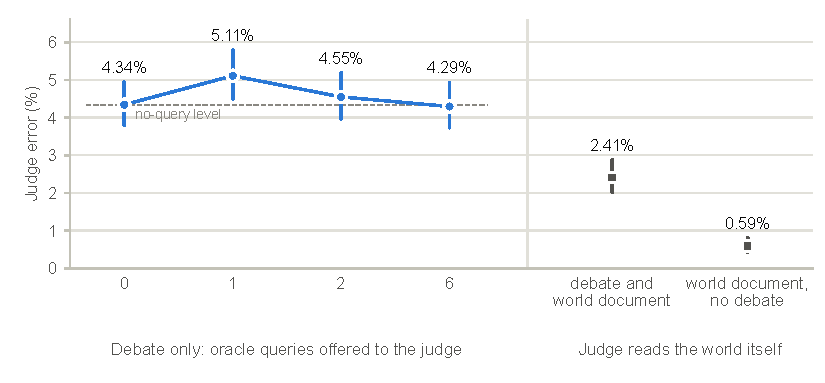
\includegraphics[width=\linewidth]{fig_error_by_arm}
\caption{Judge error in each condition, averaged over seven judges. Bars are 95\% intervals for each rate on its own;
differences between conditions are paired and more precise than overlapping bars suggest (Table~\ref{tab:arms}).
Offering one oracle query raised error a little above the no-query rate; with six offered, error was close to the
no-query rate. Judges who could read the world document made far fewer errors than judges with any number of queries.
The budgets are evenly spaced on the axis; 3 to 5 queries were not tested.}
\label{fig:arms}
\end{figure}

With no queries, judge error was \errKzero\% (Figure~\ref{fig:arms}, Table~\ref{tab:arms}). With one query offered,
it rose to \errKone\%. With two it was \errKtwo\%, and with six it was \errKsix\%, close to the no-query rate.

The rise at one query is \dOneZero{} \pp{} over no queries (95\% interval \dOneZeroCI) and \dOneSix{} \pp{} over six
queries (\dOneSixCI). Both comparisons hold, so the registered test, applied to the seven judges that produced data,
supports higher error at one query than at none and at six ($p = \pHolmOne$ after correcting for the two budgets
tested, the smallest value the procedure can return). It does not directly compare one query with two. At two queries
the differences are smaller, \dTwoZero{} and \dTwoSix{} \pp, and their intervals include zero (corrected
$p = \pHolmTwo$), so a peak at two queries is not established.

The observed peak is small in absolute terms. Before the run we set 1.5 \pp{} as the smallest peak that would matter
in practice, and under the gate as it ran the data rule out a peak that large: allowing for the several comparisons
made, the upper confidence bounds on the two differences at one query are \dOneZeroSimHi{} and \dOneSixSimHi{} \pp{}
(Appendix~\ref{app:stats}). Two things qualify ``small''. The threshold was fixed when the design required pooled
no-query error of at least 10\% in development; at the realised \errKzero\%, the rise is about \relRise\% more
errors. And the exclusion carries the same gate caveat as the peak itself (Section~\ref{sec:gate}), so we cannot say
how large the peak would be if every query had obeyed the rule.

We detected no average difference between six queries and none. Error with six queries was \dSixZero{} \pp{} lower,
with a 95\% interval from \dSixZeroLo{} \pp{} lower to \dSixZeroHi{} \pp{} higher. That average combines opposite
movements by judge (Section~\ref{sec:judges}).

\begin{table}[t]
\centering
\caption{Judge error by condition (left) and the differences between conditions (right), averaged over seven judges.
Differences are in percentage points.}
\label{tab:arms}
\footnotesize
\setlength{\tabcolsep}{4pt}
\begin{minipage}[t]{0.5\linewidth}\raggedright
\begin{tabular}{@{}lrr@{}}
\toprule
What the judge gets & Error (\%) & 95\% interval \\
\midrule
Debate, no queries & 4.34 & 3.81 to 4.94 \\
Debate, 1 query offered & 5.11 & 4.50 to 5.78 \\
Debate, 2 queries offered & 4.55 & 3.97 to 5.19 \\
Debate, 6 queries offered & 4.29 & 3.73 to 4.93 \\
\midrule
Debate and the world document & 2.41 & 2.02 to 2.87 \\
World document only, no debate & 0.59 & 0.43 to 0.81 \\
\bottomrule
\end{tabular}

\end{minipage}\hfill
\begin{minipage}[t]{0.48\linewidth}\raggedleft
\begin{tabular}{@{}lrr@{}}
\toprule
Comparison & Difference & 95\% interval \\
\midrule
1 query vs.\ none & $+0.77$ & $[+0.43,\ +1.10]$ \\
1 query vs.\ 6 & $+0.82$ & $[+0.49,\ +1.16]$ \\
2 queries vs.\ none & $+0.21$ & $[-0.06,\ +0.51]$ \\
2 queries vs.\ 6 & $+0.25$ & $[-0.04,\ +0.56]$ \\
\midrule
6 queries vs.\ none & $-0.05$ & $[-0.37,\ +0.30]$ \\
World added vs.\ 6 queries & $-1.88$ & $[-2.25,\ -1.54]$ \\
\bottomrule
\end{tabular}

\end{minipage}
\end{table}

\subsection{Reading the evidence beat querying it}
\label{sec:world}

When judges were given the world document alongside the debate, error fell to \errDebWorld\%. That is \dWorldSix{}
\pp{} lower than with six queries (95\% interval \dWorldSixCI{} lower). Under this protocol, offering up to six
queries left judges with higher error than giving them the document. Like the one-query finding, this comparison is
not robust to the gate analysis of Section~\ref{sec:gate}.

Judges who read only the world document, with no debate, erred just \errWorld\% of the time, against \errDebWorld\%
with the document and the debate. This comparison was not a registered test. Descriptively, judges made more errors
when the complete debate accompanied the document. Claude Haiku 4.5 supplies about \haikuWorldGapShare\% of that gap,
going from \errHaikuWorld\% with the document alone to \errHaikuDebWorld\% with the document and the debate. The two
conditions also differ in the judge's instructions and in how much text the judge reads, so the design does not
isolate the dishonest debater's contribution.

\subsection{Judges differed: the rise at one query was broad, the return by six was not}
\label{sec:judges}

\begin{figure}[t]
\centering
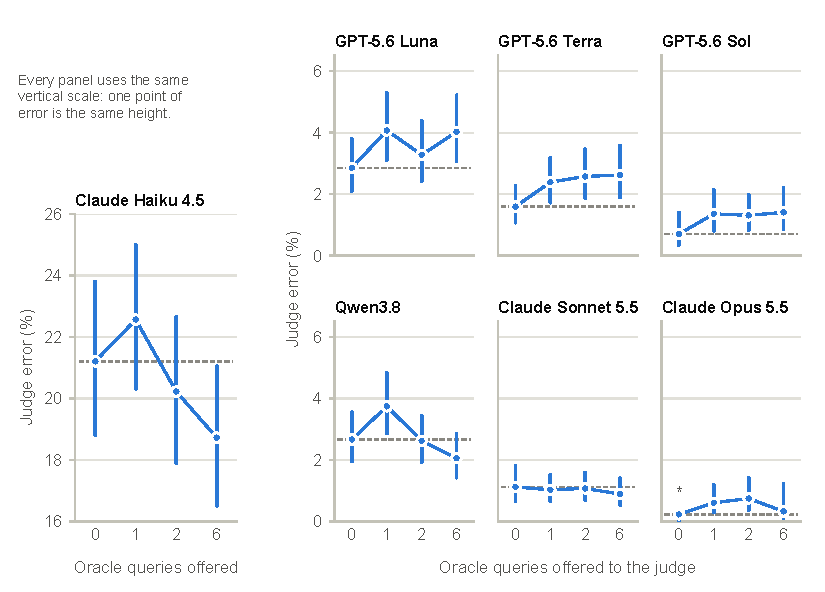
\includegraphics[width=\linewidth]{fig_error_by_judge}
\caption{Judge error by number of queries offered, for each judge. Bars are 95\% intervals for each rate on its own;
the dashed line marks each judge's no-query level. Six of seven judges erred more with one query than with none.
After that the judges part ways: the GPT-5.6 judges stayed elevated, while Haiku and Qwen3.8 ended below where they
started (for Qwen3.8, see the note on cut-off replies in the text). ($*$ this interval has no finite upper limit,
because the interval procedure breaks down when a judge makes almost no errors; only its lower part is drawn.)}
\label{fig:judges}
\end{figure}

Error was concentrated in one judge. Without queries, Claude Haiku 4.5 erred \errHaikuKzero\% of the time; the other
six judges erred between \errOthersKzeroLo\% and \errOthersKzeroHi\% (Figure~\ref{fig:judges}). Because judges count
equally, Haiku supplies about \haikuErrShare\% of the pooled error rate. With so few errors elsewhere, there was
little room for queries to improve most judges' accuracy.

The rise from none to one is broad: \nJudgesHigherAtOne{} of the seven judges erred more with one query than with
none. The exception is Sonnet 5.5, whose error barely changed (\errSonnetKzero\% to \errSonnetKone\%); it is also the
honest debater's model, and the design cannot say whether that matters. Five of seven judges' error then fell from
one query to six, though the sizes of those declines differed. The three GPT-5.6 judges were still above their
no-query level at six queries, while Haiku and Qwen3.8 ended below theirs. So the ``back down by six'' side of the
peak comes mostly from Haiku (\dHaikuOneSix{} \pp{} lower at six than at one) and Qwen3.8 (\dQwenOneSix{} \pp).
Qwen3.8's position below its no-query level needs care: \qwenCutZero{} of its no-query replies were cut off and
scored as errors, against \qwenCutSix{} with six queries (Section~\ref{sec:analysis}).

The registered check without the three Claude judges shows the same split. The estimated rise from no queries to one
remains positive and statistically supported (\ncRise{} \pp{} over the four remaining judges). The estimated decline
from one to six is smaller (\ncFall{} \pp), and the joint test for a peak does not pass the correction for testing
two budgets. This does not establish that the decline is absent. In that panel error with six queries was
\ncSixZero{} \pp{} higher than with none, a registered comparison that is not adjusted for multiple tests
(Appendix~\ref{app:stats}).

These per-judge comparisons are descriptive. Among the judges that produced data, only Qwen3.8 had registered
per-judge tests, to follow up an earlier phase; the matching tests for Llama 3.3 70B could not be run. Qwen3.8's
error rose \qwenOneZero{} \pp{} with one query (95\% interval \qwenOneZeroCI), which does not survive the registered
correction for multiple tests. That correction still counts the two Llama tests that could not be run, which makes
it stricter. Appendix~\ref{app:judges} reports how judges used their queries.

\subsection{A caveat: the gate let some rule-breaking queries through}
\label{sec:gate}

As Section~\ref{sec:oracle} explains, the gate that screened the main run failed its check of agreement with the
development gate. To see how often rule-breaking queries got through, we audited a sample of \nAuditSessions{} judge
sessions (40 per judge and budget) after the run and before any result was computed. Claude Opus 5.5 labelled every
query those sessions had sent to the gate classifier against the gate rule, without seeing the gate's decisions or
the verdicts.

About one admitted query in ten was flagged (\auditAdmittedFlaggedShare\% of \nAuditAdmitted), at much the same rate
at every budget. Sessions with more queries were therefore more likely to contain a flagged one: \exposedOne\%,
\exposedTwo\% and \exposedSix\% of sessions with one, two and six queries did. A narrower category applied to
\leakOne\%, \leakTwo\% and \leakSix\% of sessions: queries that refer to the debate or to a candidate answer, queries
that assert an answer's conclusion, and flags whose type could not be determined. The same auditor flagged
\pilotAdmFlaggedShare{} of \pilotAdmSampled{} sampled admissions of the development gate, so imperfect screening is a
property of the classifier and was not shown to come from the change of deployment (Appendix~\ref{app:gate}).

We had fixed a worst-case check for this in advance. It supposes that every session with an admitted rule-breaking
query had its verdict changed in the direction that hurts a finding, and asks how large the share of such sessions
can be before the finding is lost. The answer is very small: about \tipPeak\% of sessions in each query condition
(averaged over judges) for the one-query peak, and about \tipRuledOutOne\% for the exclusion of a 1.5-point peak,
against the 11 to 33\% of sessions the audit flagged. So we cannot rule out that rule-breaking queries contributed to
the pattern in Section~\ref{sec:peak}, in either direction. The check is also very demanding when differences are
under one point. The robustness decision uses the audit's upper bound. With \nAuditPerBudget{} sessions per budget,
even an audit with no flags would leave an upper bound of \auditZeroFlagBound\%. For the observed results, that
exceeds the tipping points for the one-query peak and the exclusions of a 1.5-point peak at one and two queries, so
all three would still fail this check. It is a bound
and not an estimate: it does not tell us how many verdicts the admitted rule-breaking queries actually changed, and
it does not show that they caused the peak. The results should be read as holding \emph{under this gate}, and as not
robust to the rule-breaking queries it admitted.

\subsection{What judges wrote in the cases that went wrong (exploratory)}
\label{sec:why}

This analysis was not registered and was designed after the results were known, so it suggests explanations and does
not test them. Appendix~\ref{app:why} has the figure, the method and its limits.

Each judge saw the same debate with no queries and with one, which gives \nPairs{} matched pairs. In \nHarm{} pairs
the judge was right without the query and wrong with it (a harmful flip); in \nHelp{} the reverse. The difference,
\nNetFlips{} pairs, is exactly the \dOneZero-point rise. The two conditions were separate runs of the judge, so a
single flip can also reflect ordinary run-to-run variation.

Four Claude Opus 5.5 sessions read the judges' written reasons in \nExplRead{} of the \nHarm{} harmful flips, chosen
by a rule fixed before reading, and labelled each case once under a written rubric. By their assessment, most
harmful flips involved a correct oracle answer followed by an unsupported conclusion: an estimated \misreadShare\%
(95\% sampling interval \misreadShareCI\%). They labelled \nOracleErrCases{} of the \nExplRead{} cases read as oracle
errors, corresponding to an estimated \oracleErrorShare\% of all harmful flips (interval \oracleErrorCI\%). Two
patterns recur. In one, the judge checks a true fact that the dishonest debater put forward, the oracle says
\textsc{yes}, and the judge treats the confirmation as support for that debater's conclusion. In the other, the
judge checks a loosely worded version of the honest debater's point, the oracle correctly says \textsc{no} or
\textsc{not addressed}, and the judge takes that as a refutation.

These readings describe the cases read and do not identify what caused the net increase. They rest on the judges'
own accounts of their reasoning; only harmful flips were read, and Haiku supplied about half of all harmful flips;
and the labels come from the oracle's own model, so shared interpretive errors could go undetected.

\subsection{Robustness}
\label{sec:robust}

The conclusions of Section~\ref{sec:peak} are unchanged when we leave out Sonnet 5.5 as a judge, leave out the two
flagged debates, or add back the two set-aside questions. Scoring the run as first registered, with the withdrawn
eighth judge counted as always wrong, gives the same conclusions by construction. On the 806 questions that drew at
most one validator flag for a possible alternative reading, the rise at one query is smaller (\detRise{} against
\dOneZero{} \pp) and still supported, and a peak at two queries is also supported.

Two checks do not support the finding, and both are described above. Without the Claude judges the joint test for a
peak at one query does not pass its correction, although the rise from none to one remains supported
(Section~\ref{sec:judges}). And the finding is not robust to the rule-breaking queries the gate admitted
(Section~\ref{sec:gate}). By the registered rule these checks are reported beside the main result and can neither
rescue nor overturn it. Appendix~\ref{app:stats} has the tables.
